%%%%%%%%%%%%%%%%%%%%%%%%%%%%%%%%%%%%%%%%%%%%%%%%%%%%%%%%%%%%%%%%
\begin{frame}[fragile]\frametitle{}
\begin{center}
{\Large ZenYoga Chapters}


{\tiny (Based on ``Zen Yoga'' by P J Saher and YouTube Channels by Abhishen, Ashish Shukla)}
\end{center}
\end{frame}


%%%%%%%%%%%%%%%%%%%%%%%%%%%%%%%%%%%%%%%%%%%%%%%%%%%%%%%%%%%%%%%%
\begin{frame}[fragile]\frametitle{}
\begin{center}
{\Large Chapter 1: Mind and Thinking}
\end{center}
\end{frame}

%%%%%%%%%%%%%%%%%%%%%%%%%%%%%%%%%%%%%%%%%%%%%%%%%%%%%%%%%%%%%%%%
\begin{frame}[fragile]\frametitle{Introduction}

\begin{itemize}
    \item The chapter discusses the mind, its thinking process, and how both interact.
    \item How thoughts influence the mind and how the mind gets distracted.
    \item Examples are provided to show how our thoughts drift and how we lose track of the original subject.
\end{itemize}

\end{frame}


%%%%%%%%%%%%%%%%%%%%%%%%%%%%%%%%%%%%%%%%%%%%%%%%%%%%%%%%%%%%%%%%
\begin{frame}[fragile]\frametitle{Types of Drifting Thoughts}

\begin{itemize}
    \item Drifting thoughts can be classified into:
    \begin{itemize}
        \item Controllable drifts
        \item Uncontrollable drifts
        \item Unrecognized drifts
    \end{itemize}
    \item Controllable drifts: When we realize the mind has drifted and we bring it back to the original subject.
    \item Uncontrollable drifts: When we completely forget the original subject and cannot recall how we got there.
\end{itemize}

\end{frame}

%%%%%%%%%%%%%%%%%%%%%%%%%%%%%%%%%%%%%%%%%%%%%%%%%%%%%%%%%%%%%%%%
\begin{frame}[fragile]\frametitle{Drifting Thoughts: Examples}

\begin{itemize}
    \item Example of controllable drift: 
        \begin{itemize}
            \item We start thinking about one subject, but our mind wanders. 
            \item Realizing the drift, we bring ourselves back to the original thought.
        \end{itemize}
    \item Example of uncontrollable drift: 
        \begin{itemize}
            \item The mind jumps from one thought to another, and eventually, we forget what we were originally thinking about.
        \end{itemize}
\end{itemize}

\end{frame}

%%%%%%%%%%%%%%%%%%%%%%%%%%%%%%%%%%%%%%%%%%%%%%%%%%%%%%%%%%%%%%%%
\begin{frame}[fragile]\frametitle{Impact of Thoughts on Actions}

\begin{itemize}
    \item Our thoughts are directly connected to our actions.
    \item Understanding the thinking process helps shape our life.
    \item If we don’t control our thoughts, we may end up in a difficult mental state.
    \item We are responsible for our thoughts, and in turn, our actions and life direction.
\end{itemize}

\end{frame}

%%%%%%%%%%%%%%%%%%%%%%%%%%%%%%%%%%%%%%%%%%%%%%%%%%%%%%%%%%%%%%%%
\begin{frame}[fragile]\frametitle{Mind and Thought Control}

\begin{itemize}
    \item If we cannot control our thoughts, it can lead to an uncontrolled mental state, or "mind drift."
    \item By understanding the nature of mind and thoughts, we can learn to control and redirect them.
    \item Meditation can help in recognizing the thought processes and bring the mind back to focus.
\end{itemize}

\end{frame}

%%%%%%%%%%%%%%%%%%%%%%%%%%%%%%%%%%%%%%%%%%%%%%%%%%%%%%%%%%%%%%%%
\begin{frame}[fragile]\frametitle{Meditation and Mind Control}

\begin{itemize}
    \item Meditation involves observing the drifting thoughts without attachment.
    \item It helps in understanding which part of the mind is active and dominant.
    \item Achieving a focused, clear state of mind is the goal of meditation.
\end{itemize}

\end{frame}

%%%%%%%%%%%%%%%%%%%%%%%%%%%%%%%%%%%%%%%%%%%%%%%%%%%%%%%%%%%%%%%%
\begin{frame}[fragile]
\frametitle{Drift Order}
\begin{itemize}
\item Drifts happen in the section of mind that deals with pictures, day-dreams.
\item Typically the come in this order:
\begin{itemize}
\item Sexual
\item Anger
\item Ego
\item Greed
\item Jealousy
\item Arrogance
\item Ignorance
\item Courage
\item Doubt
\item Day dreaming
\end{itemize}
\end{itemize}
\end{frame}


%%%%%%%%%%%%%%%%%%%%%%%%%%%%%%%%%%%%%%%%%%%%%%%%%%%%%%%%%%%%%%%%
\begin{frame}[fragile]\frametitle{Summary}

\begin{itemize}
	\item Drift: Change in thoughts away from the main subject.
	\item Types:
		\begin{itemize}
			\item Un-controllable: Unaware of it, can not recollect
			\item Controllable: Can detect and come back to the main subject.
		\end{itemize}
	\item Mind, if not trained, can not channelize drifts.
	\item This drift is not property of the whole mind but one section within it.
	\item So, learn to separate sections of mind and understand the functionality.
    \item Understanding mind and thought drifts is essential for self-awareness and personal growth.
    \item Thoughts lead to actions, and actions shape our lives.
    \item Meditation and mindfulness can help control the mind and direct it towards constructive actions.
    \item Mastery over thoughts leads to a harmonious and controlled life.
\end{itemize}

\end{frame}

%%%%%%%%%%%%%%%%%%%%%%%%%%%%%%%%%%%%%%%%%%%%%%%%%%%%%%%%%%%%%%%%
\begin{frame}[fragile]\frametitle{}
\begin{center}
{\Large Chapter 2: Drifts of the Mind and What they convey?}
\end{center}
\end{frame}


%%%%%%%%%%%%%%%%%%%%%%%%%%%%%%%%%%%%%%%%%%%%%%%%%%%%%%%%%%%%%%%%
\begin{frame}[fragile]\frametitle{Introduction}
  \begin{itemize}
    \item This chapter focuses on three main concepts in Zenyoga: Simple Consciousness, Self-Consciousness, and Cosmic Consciousness.
    \item Simple Consciousness: Present in all living beings, including animals and humans.
    \item Self-Consciousness: Exclusive to humans, which helps us observe and control our mind's state.
    \item Cosmic Consciousness: A higher state of awareness that transcends individual identity.
  \end{itemize}
\end{frame}

%%%%%%%%%%%%%%%%%%%%%%%%%%%%%%%%%%%%%%%%%%%%%%%%%%%%%%%%%%%%%%%%
\begin{frame}[fragile]\frametitle{Simple Consciousness}
  \begin{itemize}
    \item Simple consciousness is a state present in all living beings.
    \item It allows us to be aware of our surroundings and react accordingly.
    \item This awareness is crucial for survival and adaptation to the environment.
    \item Animals also experience simple consciousness but lack the ability to reflect on their mental states.
  \end{itemize}
\end{frame}

%%%%%%%%%%%%%%%%%%%%%%%%%%%%%%%%%%%%%%%%%%%%%%%%%%%%%%%%%%%%%%%%
\begin{frame}[fragile]\frametitle{Self-Consciousness}
  \begin{itemize}
    \item Self-consciousness is unique to humans, allowing us to reflect on and control our mental states.
    \item Humans can observe their mood swings and emotions throughout the day.
    \item This ability to reflect and evolve one's mind is a key aspect of human nature.
    \item Unlike animals, humans can identify their identity and separate it from the environment.
  \end{itemize}
\end{frame}

%%%%%%%%%%%%%%%%%%%%%%%%%%%%%%%%%%%%%%%%%%%%%%%%%%%%%%%%%%%%%%%%
\begin{frame}[fragile]\frametitle{Challenges in Self-Consciousness}
  \begin{itemize}
    \item While humans have the potential for self-awareness, it is often difficult to concentrate and meditate.
    \item Our comfort zone and habits prevent us from evolving our minds effectively.
    \item The difficulty lies in sustaining concentration and overcoming habitual patterns.
  \end{itemize}
\end{frame}

%%%%%%%%%%%%%%%%%%%%%%%%%%%%%%%%%%%%%%%%%%%%%%%%%%%%%%%%%%%%%%%%
\begin{frame}[fragile]\frametitle{Cosmic Consciousness}
  \begin{itemize}
    \item Cosmic consciousness is a higher state of awareness that transcends individual identity.
    \item It is a state where one feels a deep connection with the universe.
    \item Achieving this state requires overcoming the distractions of the mind and focusing on a higher subject.
    \item It is a state that few have achieved due to the complexity of human tendencies.
  \end{itemize}
\end{frame}

%%%%%%%%%%%%%%%%%%%%%%%%%%%%%%%%%%%%%%%%%%%%%%%%%%%%%%%%%%%%%%%%
\begin{frame}[fragile]\frametitle{The Story of Narada and Krishna}
  \begin{itemize}
    \item Narada Muni asks Lord Krishna why humans remain trapped in the illusion of the physical world.
    \item Krishna explains that humans have the potential to achieve enlightenment but are distracted by the mind’s tendencies.
    \item Narada Muni forgets his mission to bring water for Krishna after being distracted by a woman at the river.
    \item The woman reveals herself to be Krishna, demonstrating how even enlightened beings can be distracted by worldly matters.
  \end{itemize}
\end{frame}



%%%%%%%%%%%%%%%%%%%%%%%%%%%%%%%%%%%%%%%%%%%%%%%%%%%%%%%%%%%%%%%%
\begin{frame}[fragile]\frametitle{Exercise}
\begin{itemize}
\item Put aside 15-30 minutes in a day to watch the drifts and note them down.
\item Take one thought as the main subject.
\item Let the mind drift.
\item Classify and note the drift.
\item Never try to make your mind ``blank''.
\item Analyze over 3 months, the persistent patterns.
\item After 15 days of consistent practice, you will start recognizing which mental centers dominate your mind.
\item Over time, this awareness will help you overcome mental distractions and develop a deeper connection with the 
\end{itemize}
\end{frame}




%%%%%%%%%%%%%%%%%%%%%%%%%%%%%%%%%%%%%%%%%%%%%%%%%%%%%%%%%%%%%%%%
\begin{frame}[fragile]\frametitle{Summary}
Forms of Consciousness:
\begin{itemize}
\item Simple: like animals, awareness of body. Needed for daily survival.
\item Self: Aware of mental states, sense of self, thoughts.
\item Cosmic: Higher state. Not achieved by logic, reasoning, etc but by stronger awareness.
\item No one has shown practical steps to go from Self to Cosmic consciousness.
\item Even if we get to know the steps, they are difficult to follow. Old patterns are hard to break away from.
\item The journey from simple consciousness to cosmic consciousness is challenging but achievable with dedication.
\item Regular practice, patience, and awareness are key to evolving the mind and reaching higher states of consciousness.
\item Zenyoga provides tools to understand and transcend the mind's limitations, leading to enlightenment.
\end{itemize}


\end{frame}


%%%%%%%%%%%%%%%%%%%%%%%%%%%%%%%%%%%%%%%%%%%%%%%%%%%%%%%%%%%%%%%%
\begin{frame}[fragile]\frametitle{}
\begin{center}
{\Large Chapter 3: What is the Mind of Man}
\end{center}
\end{frame}

%%%%%%%%%%%%%%%%%%%%%%%%%%%%%%%%%%%%%%%%%%%%%%%%%%%%%%%%%%%%%%%%
\begin{frame}[fragile]\frametitle{Introduction to Mind and Brain}
\begin{itemize}
    \item \textbf{Mind vs. Brain:} Saher explains that the mind is not equivalent to the physical brain.
    \item The \textbf{mind} is an accumulation of thoughts, while the \textbf{brain} processes these thoughts through sensory inputs.
    \item The brain uses sensory inputs (five senses) to capture, process, and decode external impulses, leading to personal interpretations.
\end{itemize}
\end{frame}

%%%%%%%%%%%%%%%%%%%%%%%%%%%%%%%%%%%%%%%%%%%%%%%%%%%%%%%%%%%%%%%%
\begin{frame}[fragile]\frametitle{Individual Interpretation and Perception}
\begin{itemize}
    \item Each individual interprets external impulses differently based on personal background, environment, and previous experiences.
    \item \textbf{Unique Interpretations:} No two people perceive an event in the exact same way; similar to how people react differently to the same movie.
    \item The mind remains \textbf{invisible}, as it is a collection of thoughts, making self-observation challenging yet essential.
\end{itemize}
\end{frame}

%%%%%%%%%%%%%%%%%%%%%%%%%%%%%%%%%%%%%%%%%%%%%%%%%%%%%%%%%%%%%%%%
\begin{frame}[fragile]\frametitle{Self-Understanding and Observation}
\begin{itemize}
    \item \textbf{Self-Observation:} Observing and understanding one’s thoughts is necessary to understand one's mind.
    \item Modern individuals often lack the time or willingness to introspect, limiting their understanding of themselves and others.
    \item Saher emphasizes that \textbf{self-reflection} enables clarity in understanding both oneself and others.
\end{itemize}
\end{frame}

%%%%%%%%%%%%%%%%%%%%%%%%%%%%%%%%%%%%%%%%%%%%%%%%%%%%%%%%%%%%%%%%
\begin{frame}[fragile]\frametitle{Connection with Others’ Minds}
\begin{itemize}
    \item Saher describes three possibilities when minds interact:
    \begin{itemize}
        \item \textbf{Affinity:} Similar thoughts lead to friendship, love, or positive relationships.
        \item \textbf{Repulsion:} Differences in thought can lead to disagreement, negativity, and hostility.
        \item \textbf{Indifference:} Lack of emotional reaction, potentially leading to detachment or even depression.
    \end{itemize}
\end{itemize}
\end{frame}

%%%%%%%%%%%%%%%%%%%%%%%%%%%%%%%%%%%%%%%%%%%%%%%%%%%%%%%%%%%%%%%%
\begin{frame}[fragile]\frametitle{The Nature of Mind and Emotions}

\begin{itemize}
    \item Saher likens the mind to a \textbf{fabric woven from various thoughts}, colored by emotions.
    \item \textbf{Emotions} act as dyes, influencing the overall tone of the mind.
    \item \textbf{Habits and Patterns:} Positive habits strengthen the mind, while emotional quality affects its openness, resilience, and overall character.
\end{itemize}
\end{frame}

%%%%%%%%%%%%%%%%%%%%%%%%%%%%%%%%%%%%%%%%%%%%%%%%%%%%%%%%%%%%%%%%
\begin{frame}[fragile]
\frametitle{Mind as a Cloth}
\begin{itemize}
\item Thoughts are strands
\item Emotions are the colors
\item Repetition or habit strengthens and makes cloth durable.
\item Quality of thoughts correspond to smoothness or roughness of the cloth.
\item Grey matter, attitude, thought process: Shape of the cloth
\item Likes/Dislikes: fashion of the cloth.
\end{itemize}

Constant daily practice can change the properties of the cloth.
\end{frame}

%%%%%%%%%%%%%%%%%%%%%%%%%%%%%%%%%%%%%%%%%%%%%%%%%%%%%%%%%%%%%%%%
\begin{frame}[fragile]\frametitle{The Influence of Thoughts on Personality}

\begin{itemize}
    \item Thoughts accumulate over time, shaping \textbf{personality} and \textbf{character}.
    \item \textbf{Intelligence and Reflection:} Using intelligence helps define character by understanding and refining thoughts.
    \item Individual perception shapes how external impulses are decoded, reinforcing unique mental patterns.
\end{itemize}
\end{frame}

%%%%%%%%%%%%%%%%%%%%%%%%%%%%%%%%%%%%%%%%%%%%%%%%%%%%%%%%%%%%%%%%
\begin{frame}[fragile]\frametitle{Importance of Self-Observation}

\begin{itemize}
    \item Saher encourages \textbf{watching and understanding one's mental patterns}.
    \item Ancient sages could observe both their own and others' thoughts, achieving clarity and wisdom.
    \item Self-awareness helps to evolve one's mind and break free from repetitive thought patterns.
\end{itemize}
\end{frame}

%%%%%%%%%%%%%%%%%%%%%%%%%%%%%%%%%%%%%%%%%%%%%%%%%%%%%%%%%%%%%%%%
\begin{frame}[fragile]\frametitle{Patterns and Automatic Reactions}

\begin{itemize}
    \item Most individuals are \textbf{reactive}, like a tape recorder, responding automatically to stimuli.
    \item External stimuli often govern behavior without conscious understanding.
    \item \textbf{Key to Self-Control:} Observation allows individuals to move from reaction to conscious response.
\end{itemize}
\end{frame}



%%%%%%%%%%%%%%%%%%%%%%%%%%%%%%%%%%%%%%%%%%%%%%%%%%%%%%%%%%%%%%%%
\begin{frame}[fragile]\frametitle{Chapter 3 Summary}
	\begin{itemize}
	\item Brain is a physical entity.
	\item Impulses come from various sensory organs, which perturb the nerves/areas in brain. These are called as `thoughts'.
	\item Collection of thoughts (or the software/platform, in IMHO) is called as `mind'.
	\item Reactions to other minds can be of types:
		\begin{itemize}
			\item Affinity: love
			\item Repulsion: hate
			\item Indifference
		\end{itemize}
	\end{itemize}

\end{frame}




%%%%%%%%%%%%%%%%%%%%%%%%%%%%%%%%%%%%%%%%%%%%%%%%%%%%%%%%%%%%%%%%
\begin{frame}[fragile]\frametitle{}
\begin{center}
{\Large Chapter 4: Do We Think and How?}
\end{center}
\end{frame}


%%%%%%%%%%%%%%%%%%%%%%%%%%%%%%%%%%%%%%%%%%%%%%%%%%%%%%%%%%%%%%%%
\begin{frame}[fragile]\frametitle{Key Concepts of Mind's Impulse Reception and Decoding}
    \begin{itemize}
        \item The mind receives external impulses and decodes them rapidly.
        \item These impulses are registered in specific areas of the brain.
        \item Each person's interpretation and reaction to the same impulse varies.
        \item Influencing factors include: Culture, character, education, circumstances, surroundings, and health.
    \end{itemize}
\end{frame}

%%%%%%%%%%%%%%%%%%%%%%%%%%%%%%%%%%%%%%%%%%%%%%%%%%%%%%%%%%%%%%%%
\begin{frame}[fragile]\frametitle{The Influence of Personal Filters on Thoughts and Actions}
    \begin{itemize}
        \item Impulses registered in the mind start as \textbf{pure mental energy}.
        \item This energy, unaltered initially, becomes modified when interpreted.
        \item Personal characteristics and surroundings color this interpretation.
        \item Thoughts impact personality, mental health, and actions significantly.
    \end{itemize}
\end{frame}

%%%%%%%%%%%%%%%%%%%%%%%%%%%%%%%%%%%%%%%%%%%%%%%%%%%%%%%%%%%%%%%%
\begin{frame}[fragile]\frametitle{Four States of Impulse Processing}
    \begin{itemize}
        \item \textbf{Pure Mental Energy State}: Initial state, unaltered and unprocessed.
        \item \textbf{Thought-Free Symbolic State}: Registered but remains unexpressed in words or images.
        \item \textbf{Mental Imagery State}: Formulated into mental images or daydreaming states.
        \item \textbf{Expressed State in Actions}: Converted into physical actions and expressions.
    \end{itemize}
\end{frame}

%%%%%%%%%%%%%%%%%%%%%%%%%%%%%%%%%%%%%%%%%%%%%%%%%%%%%%%%%%%%%%%%
\begin{frame}[fragile]\frametitle{Understanding Intention vs. Action}
    \begin{itemize}
        \item True actions are judged by intentions, not merely outward expressions.
        \item Actions may not always convey underlying intentions.
        \item Importance of internal purity over external validation.
    \end{itemize}
\end{frame}

%%%%%%%%%%%%%%%%%%%%%%%%%%%%%%%%%%%%%%%%%%%%%%%%%%%%%%%%%%%%%%%%
\begin{frame}[fragile]\frametitle{Insights from Patanjali's Yogasutra}
    \begin{itemize}
        \item Five states of mind affecting pleasure or pain.
        \item Practices like \textbf{Non-attachment} help control mental fluctuations.
        \item \textbf{Constant Effort} (तपस्) is essential to restrain negative modifications.
        \item \textbf{Purification} of mind leads to clarity and cosmic consciousness.
    \end{itemize}
\end{frame}

%%%%%%%%%%%%%%%%%%%%%%%%%%%%%%%%%%%%%%%%%%%%%%%%%%%%%%%%%%%%%%%%
\begin{frame}[fragile]\frametitle{Path to Pure Mind and Cosmic Consciousness}
    \begin{itemize}
        \item Remove filters to perceive the true nature of impulses.
        \item Modifications act as filters, limiting pure awareness.
        \item Pure awareness emerges when filters are removed.
        \item Expanding awareness leads towards cosmic consciousness.
    \end{itemize}
\end{frame}



%%%%%%%%%%%%%%%%%%%%%%%%%%%%%%%%%%%%%%%%%%%%%%%%%%%%%%%%%%%%%%%%
\begin{frame}[fragile]\frametitle{Chapter 4 Summary}
	\begin{itemize}
	\item Incoming impulses are decoded in brain as Pure Mind Energy, which are divided into:
		\begin{itemize}
			\item Held: thoughts suppressed
			\item Words: expressed as words or mental pictures, day dreaming.
			\item Actions: Something is done by them, movements.
		\end{itemize}
	\item As per Patanjali पतंजली , there are 5 states (`vrutti' वृत्ती ) of mind (`chitta' चित्त ):
		\begin{itemize}
			\item Correct Knowledge
			\item Incorrect Knowledge
			\item Fancy
			\item Passivity (sleep)
			\item Memory
		\end{itemize}
	\item Mind can be controlled (``chitta vrutti nirodh:'' चित्त वृत्ती निरोध ) by efforts, detachment.
	\item Peace of mind can be brought by regulation of ``prana'' प्राण (breath).
	\item Mental purification and clarity are keys to true perception.
	\item Detaching from modifications allows pure awareness to arise.
	\item Regular practice leads to cosmic consciousness and expansive awareness.	
	\end{itemize}

\end{frame}

%%%%%%%%%%%%%%%%%%%%%%%%%%%%%%%%%%%%%%%%%%%%%%%%%%%%%%%%%%%%%%%%
\begin{frame}[fragile]\frametitle{}
\begin{center}
{\Large Chapter 5: Must We Sleep and How Much?}
\end{center}
\end{frame}

%%%%%%%%%%%%%%%%%%%%%%%%%%%%%%%%%%%%%%%%%%%%%%%%%%%%%%%%%%%%%%%%
\begin{frame}[fragile]\frametitle{Must-Read on Sleep and Its Importance}
    \begin{itemize}
        \item Sleep is essential, but managing energy efficiently can reduce the hours needed.
        \item Saher compares sleep to income: well-managed sleep conserves mental and physical energy.
        \item Overuse of energy in unnecessary activities leads to a need for more sleep.
    \end{itemize}
\end{frame}

%%%%%%%%%%%%%%%%%%%%%%%%%%%%%%%%%%%%%%%%%%%%%%%%%%%%%%%%%%%%%%%%
\begin{frame}[fragile]\frametitle{Different Types of Sleep}
    \begin{itemize}
        \item Saher categorizes sleep based on its timing and impact:
        \begin{itemize}
            \item \textbf{12am - 4am:} Most beneficial, replenishing energy.
            \item \textbf{11pm - 5am:} Intense and beneficial, suitable for restful sleep.
            \item \textbf{9pm - 11pm \& 5am - 7am:} Neutral sleep, provides minimal energy.
            \item \textbf{7am - 12pm:} Wastes energy, leaves one feeling tired.
            \item \textbf{12pm - 4pm:} Can harm health by depleting vital energy.
            \item \textbf{4pm - 9pm:} Damaging, attracts negative energy and illnesses.
        \end{itemize}
    \end{itemize}
\end{frame}

%%%%%%%%%%%%%%%%%%%%%%%%%%%%%%%%%%%%%%%%%%%%%%%%%%%%%%%%%%%%%%%%
\begin{frame}[fragile]\frametitle{Benefits of Reducing Sleep Hours}
    \begin{itemize}
        \item By reducing sleep to around 6 hours, one can gain 2-3 extra productive hours daily.
        \item Extra time can be spent on creative pursuits, learning new skills, and meditation.
        \item Saher encourages less sleep to engage more in life's constructive activities.
    \end{itemize}
\end{frame}

%%%%%%%%%%%%%%%%%%%%%%%%%%%%%%%%%%%%%%%%%%%%%%%%%%%%%%%%%%%%%%%%
\begin{frame}[fragile]\frametitle{Meditation and Energy Regulation}
    \begin{itemize}
        \item Meditation benefits those who regulate energy and daily activities effectively.
        \item Saher emphasizes moderation in food, recreation, and sleep as keys to happiness.
        \item Excess sleep or too little regulation can disrupt inner peace and hamper meditation.
    \end{itemize}
\end{frame}


%%%%%%%%%%%%%%%%%%%%%%%%%%%%%%%%%%%%%%%%%%%%%%%%%%%%%%%%%%%%%%%%
\begin{frame}[fragile]\frametitle{Summary}

	\begin{itemize}
	\item Types of Sleep are:
	
		\resizebox{\textwidth}{!}{%
		  \begin{tabular}{|c|c|c|c|c|}
		  \hline
		  Type & Beneficial? & Timing& Vibrational Color built in Body\\
		  \hline
		  Very Intense 	& 	Very beneficial	&	Midnight to 4am	&	Pale Blue\\
		  Intense     	&	Beneficial		& 	11pm to Midnight, 4 to 5am	&	Pink\\
		  Indifferent  	&	Does not add to energy	& 9 to 11pm, 5 to 7am &Green\\
		  Wasting		& 	Losing energy & 7am to 12 noon & Yellow (dark) \\
		  Damaging		& 	Bad to nerves &  12 noon to 4 pm & Orange (deep)\\
		  Highly Damaging & Sickness, disease & 4pm to 9pm&  Red (deep)\\
		  \hline
		  \end{tabular}
		} % end of scope of "\resizebox"  directive

	\item Resting and sleeping are two different things.
	\item 11pm to 5pm should be considered as a good time for sleep.
	\end{itemize}
\end{frame}


%%%%%%%%%%%%%%%%%%%%%%%%%%%%%%%%%%%%%%%%%%%%%%%%%%%%%%%%%%%%%%%%
\begin{frame}[fragile]\frametitle{}
\begin{center}
{\Large Chapter 6: Expanding Consciousness}
\end{center}
\end{frame}

%%%%%%%%%%%%%%%%%%%%%%%%%%%%%%%%%%%%%%%%%%%%%%%%%%%%%%%%%%%%%%%%
\begin{frame}[fragile]\frametitle{Expanding Consciousness}
    \begin{itemize}
        \item Interrelation of \textbf{Life}, \textbf{Body}, and \textbf{Consciousness}
        \item Awareness cannot be fully understood without life and vice versa
        \item Connection of subtle body (सुक्ष्म शरीर) to physical form and experiences
    \end{itemize}
\end{frame}

%%%%%%%%%%%%%%%%%%%%%%%%%%%%%%%%%%%%%%%%%%%%%%%%%%%%%%%%%%%%%%%%
\begin{frame}[fragile]\frametitle{Levels of Consciousness Across Beings}
    \begin{itemize}
        \item Varying levels of consciousness in minerals, plants, animals, and humans
        \item Humans possess a unique ability to perceive self-identity and consciousness
        \item Intelligence is perceived highest in humans, viewing themselves as distinct in the universe
    \end{itemize}
\end{frame}

%%%%%%%%%%%%%%%%%%%%%%%%%%%%%%%%%%%%%%%%%%%%%%%%%%%%%%%%%%%%%%%%
\begin{frame}[fragile]\frametitle{Sleep and Consciousness}
    \begin{itemize}
        \item Sleep disconnects conscious awareness, yet bodily functions persist
        \item During sleep, life force continues essential functions (e.g., heartbeat, digestion)
        \item Waking after sleep brings an un-explainable sense of refreshment and rest
    \end{itemize}
\end{frame}

%%%%%%%%%%%%%%%%%%%%%%%%%%%%%%%%%%%%%%%%%%%%%%%%%%%%%%%%%%%%%%%%
\begin{frame}[fragile]\frametitle{Divine Potential in Humans}
    \begin{itemize}
        \item Human life, consciousness, and physical body together shape divine potential
        \item Realizing divinity requires heightened awareness and understanding of one’s consciousness
        \item Observing differences between light and darkness as metaphors for awareness
    \end{itemize}
\end{frame}

%%%%%%%%%%%%%%%%%%%%%%%%%%%%%%%%%%%%%%%%%%%%%%%%%%%%%%%%%%%%%%%%
\begin{frame}[fragile]\frametitle{Color of Aura Based on Sleep Patterns}
    \begin{itemize}
        \item \textbf{Blue Aura}: Sleep from 12 AM - 4 AM
        \item \textbf{Pink Aura}: Sleep from 11 PM - 5 AM
        \item \textbf{Green Aura}: Sleep from 9 PM - 11 PM and wake by 5 AM
        \item \textbf{Yellow Aura}: Sleep from 7 AM - 12 PM (can deplete energy)
        \item \textbf{Orange Aura}: Sleep from 12 PM - 4 PM (risk of health issues)
        \item \textbf{Red Aura}: Sleep from 4 PM - 9 PM (associated with negative energies)
    \end{itemize}
\end{frame}

%%%%%%%%%%%%%%%%%%%%%%%%%%%%%%%%%%%%%%%%%%%%%%%%%%%%%%%%%%%%%%%%
\begin{frame}[fragile]\frametitle{Reflective Question}
    \begin{itemize}
        \item ``What is the impact of sleep on vital functions?''
        \item Encouragement to ponder the unseen forces that sustain life during sleep
    \end{itemize}
\end{frame}

%%%%%%%%%%%%%%%%%%%%%%%%%%%%%%%%%%%%%%%%%%%%%%%%%%%%%%%%%%%%%%%%
\begin{frame}[fragile]\frametitle{}
\begin{center}
{\Large Chapter 7: Breathing and It's Relationship to Consciousness and Life}
\end{center}
\end{frame}

%%%%%%%%%%%%%%%%%%%%%%%%%%%%%%%%%%%%%%%%%%%%%%%%%%%%%%%%%%%%%%%%
\begin{frame}[fragile]\frametitle{Breathing and Life Relationship}
    \begin{itemize}
        \item Breathing is not just inhaling oxygen but is essential for life.
        \item The essence of life begins with the breath and ends with it.
        \item Breathing influences our mind and actions through coded impulses.
    \end{itemize}
\end{frame}

%%%%%%%%%%%%%%%%%%%%%%%%%%%%%%%%%%%%%%%%%%%%%%%%%%%%%%%%%%%%%%%%
\begin{frame}[fragile]\frametitle{Breath as a Source of Impulses}
    \begin{itemize}
        \item Breath brings coded impulses that the mind decodes to create thoughts.
        \item These impulses are received not only from breath but also through food, touch, and senses.
        \item Mind processes these impulses, leading to thoughts and actions.
    \end{itemize}
\end{frame}

%%%%%%%%%%%%%%%%%%%%%%%%%%%%%%%%%%%%%%%%%%%%%%%%%%%%%%%%%%%%%%%%
\begin{frame}[fragile]\frametitle{Hunger Beyond Food}
    \begin{itemize}
        \item Just as we hunger for food, we have emotional and sexual appetites.
        \item Regulating these appetites is essential for spiritual progress.
        \item Overindulgence in any impulse leads to entanglement in worldly illusions.
    \end{itemize}
\end{frame}

%%%%%%%%%%%%%%%%%%%%%%%%%%%%%%%%%%%%%%%%%%%%%%%%%%%%%%%%%%%%%%%%
\begin{frame}[fragile]\frametitle{Avoiding Overindulgence}
    \begin{itemize}
        \item Overindulgence in impulses (food, touch, etc.) disrupts spiritual growth.
        \item Pure willpower alone is insufficient to control these impulses.
        \item Developing good habits gradually helps regulate these impulses effectively.
    \end{itemize}
\end{frame}

%%%%%%%%%%%%%%%%%%%%%%%%%%%%%%%%%%%%%%%%%%%%%%%%%%%%%%%%%%%%%%%%
\begin{frame}[fragile]\frametitle{Developing Patience}
    \begin{itemize}
        \item Patience is key for overcoming bad habits and progressing spiritually.
        \item Saher explains that adopting good habits requires i-centre involvement.
        \item Bad habits are easy to adopt as they don’t require much effort from the i-centre.
    \end{itemize}
\end{frame}

%%%%%%%%%%%%%%%%%%%%%%%%%%%%%%%%%%%%%%%%%%%%%%%%%%%%%%%%%%%%%%%%
\begin{frame}[fragile]\frametitle{Pleasure vs. Pain}
    \begin{itemize}
        \item Pleasures can turn into pain in the long run (e.g., consuming sugary foods).
        \item Some pleasures offer momentary enjoyment but harm overall health.
        \item Practicing awareness helps discern between beneficial and harmful pleasures.
    \end{itemize}
\end{frame}

%%%%%%%%%%%%%%%%%%%%%%%%%%%%%%%%%%%%%%%%%%%%%%%%%%%%%%%%%%%%%%%%
\begin{frame}[fragile]\frametitle{Self-Regulation and Spiritual Evolution}
    \begin{itemize}
        \item Humans have free will to make choices for long-term health and mental clarity.
        \item Staying mindful of impulses aids in evolving towards one’s full potential.
        \item Saher suggests focusing on self-growth rather than chasing fleeting pleasures.
    \end{itemize}
\end{frame}

%%%%%%%%%%%%%%%%%%%%%%%%%%%%%%%%%%%%%%%%%%%%%%%%%%%%%%%%%%%%%%%%
\begin{frame}[fragile]\frametitle{Summary}
    \begin{itemize}
        \item Breathing and impulses play a vital role in shaping thoughts and actions.
        \item Developing awareness and good habits enables spiritual progress.
        \item Saher advocates integrating breathing regulation with life’s purpose.
    \end{itemize}
\end{frame}

%%%%%%%%%%%%%%%%%%%%%%%%%%%%%%%%%%%%%%%%%%%%%%%%%%%%%%%%%%%%%%%%
\begin{frame}[fragile]\frametitle{}
\begin{center}
{\Large Chapter 8: Spiritual Planes}
\end{center}
\end{frame}

%%%%%%%%%%%%%%%%%%%%%%%%%%%%%%%%%%%%%%%%%%%%%%%%%%%%%%%%%%%%%%%%
\begin{frame}[fragile]\frametitle{Spiritual Planes}
    \begin{itemize}
        \item Chapter 8 of the book focuses on spiritual planes and their significance.
        \item The chapter addresses common questions that might arise in the spiritual journey.
    \end{itemize}
\end{frame}

%%%%%%%%%%%%%%%%%%%%%%%%%%%%%%%%%%%%%%%%%%%%%%%%%%%%%%%%%%%%%%%%
\begin{frame}[fragile]\frametitle{Five Factors Affecting Spiritual Growth}
    \begin{itemize}
        \item Our five senses help us perceive and react to external stimuli.
        \item These factors influence our spiritual journey and need regulation:
            \begin{itemize}
                \item Breathing
                \item Food and Drink
                \item External Sensory Input
                \item Sleep or Inertia
                \item Sex
            \end{itemize}
    \end{itemize}
\end{frame}

%%%%%%%%%%%%%%%%%%%%%%%%%%%%%%%%%%%%%%%%%%%%%%%%%%%%%%%%%%%%%%%%
\begin{frame}[fragile]\frametitle{Preparing for Critical Stages}
    \begin{itemize}
        \item To reach a critical stage in spirituality, the body and mind must be ready.
        \item Superficial practices or shortcuts may not sustain this stage and can harm the body and mind.
    \end{itemize}
\end{frame}

%%%%%%%%%%%%%%%%%%%%%%%%%%%%%%%%%%%%%%%%%%%%%%%%%%%%%%%%%%%%%%%%
\begin{frame}[fragile]\frametitle{Pratyahara: The Stage of Withdrawal}
    \begin{itemize}
        \item The critical spiritual stage aligns with the concept of \textbf{Pratyahara} प्रत्याहार in Yoga.
        \item This stage follows yama यम  , niyam नियम , asan आसन , pranayam प्राणायाम 
        \item Mastering prior practices is essential to sustain the critical stage.
    \end{itemize}
\end{frame}

%%%%%%%%%%%%%%%%%%%%%%%%%%%%%%%%%%%%%%%%%%%%%%%%%%%%%%%%%%%%%%%%
\begin{frame}[fragile]\frametitle{Importance of Awareness in Daily Life}
    \begin{itemize}
        \item Daily awareness in thoughts, diet, and actions is crucial.
        \item Simply meditating for a short time daily is insufficient.
        \item A disciplined lifestyle enables one to sustain the critical stage.
    \end{itemize}
\end{frame}

%%%%%%%%%%%%%%%%%%%%%%%%%%%%%%%%%%%%%%%%%%%%%%%%%%%%%%%%%%%%%%%%
\begin{frame}[fragile]\frametitle{Role of a Physical Guru}
    \begin{itemize}
        \item A physical guru can provide guidance but cannot evolve one’s mind directly.
        \item Genuine progress in spirituality requires personal effort and self-awareness.
    \end{itemize}
\end{frame}

%%%%%%%%%%%%%%%%%%%%%%%%%%%%%%%%%%%%%%%%%%%%%%%%%%%%%%%%%%%%%%%%
\begin{frame}[fragile]\frametitle{The Spiritual Master Appears}
    \begin{itemize}
        \item ``When the disciple is ready, the master will appear'' - a profound idea.
        \item The real master may not be a physical entity but a divine guiding light.
    \end{itemize}
\end{frame}

%%%%%%%%%%%%%%%%%%%%%%%%%%%%%%%%%%%%%%%%%%%%%%%%%%%%%%%%%%%%%%%%
\begin{frame}[fragile]\frametitle{Preparation for Higher Guidance}
    \begin{itemize}
        \item Self-discipline and readiness are essential for receiving divine guidance.
        \item The practices in the book encourage evolving mind and body for critical stages.
    \end{itemize}
\end{frame}

%%%%%%%%%%%%%%%%%%%%%%%%%%%%%%%%%%%%%%%%%%%%%%%%%%%%%%%%%%%%%%%%
\begin{frame}[fragile]\frametitle{Summary}
    \begin{itemize}
        \item Spiritual evolution impacts all aspects of life, enhancing creativity and awareness.
        \item The practices help in realizing our divine nature, enriching life and relationships.
    \end{itemize}
\end{frame}


%%%%%%%%%%%%%%%%%%%%%%%%%%%%%%%%%%%%%%%%%%%%%%%%%%%%%%%%%%%%%%%%
\begin{frame}[fragile]\frametitle{}
\begin{center}
{\Large Chapter 9: Avoidable Mistakes }
\end{center}
\end{frame}

%%%%%%%%%%%%%%%%%%%%%%%%%%%%%%%%%%%%%%%%%%%%%%%%%%%%%%%%%%%%%%%%
\begin{frame}[fragile]\frametitle{Introduction to Mind Regulation}
    \begin{itemize}
        \item Mind regulation helps us proceed in life and make sound decisions.
        \item It's essential to understand and control the mind’s energy.
        \item Share this knowledge with your loved ones to help them regulate their minds too.
    \end{itemize}
\end{frame}

%%%%%%%%%%%%%%%%%%%%%%%%%%%%%%%%%%%%%%%%%%%%%%%%%%%%%%%%%%%%%%%%
\begin{frame}[fragile]\frametitle{Mind and Self}
    \begin{itemize}
        \item Our body and self are distinct entities.
        \item We invest in decorating the physical body, though it’s temporary.
        \item True focus should be on the eternal inner self, which transcends physical limitations.
    \end{itemize}
\end{frame}

%%%%%%%%%%%%%%%%%%%%%%%%%%%%%%%%%%%%%%%%%%%%%%%%%%%%%%%%%%%%%%%%
\begin{frame}[fragile]\frametitle{The Self and Mind Centers}
    \begin{itemize}
        \item The self is symbolized as a ``Chairman'' with two ``Managing Directors'':
        \begin{itemize}
            \item Senior Managing Director: Transcendental Center
            \item Junior Managing Director: Para Mental Center
        \end{itemize}
        \item Five directors under them represent five centers of the mind.
    \end{itemize}
\end{frame}

%%%%%%%%%%%%%%%%%%%%%%%%%%%%%%%%%%%%%%%%%%%%%%%%%%%%%%%%%%%%%%%%
\begin{frame}[fragile]\frametitle{The Five Centers of the Mind}
    \begin{itemize}
        \item \textbf{'I' Center}: Guides decision-making; represents clarity.
        \item \textbf{'E' Center}: Generates crude and noble emotions.
        \item \textbf{'S' Center}: Governs biological Sex instincts and responses.
        \item \textbf{'M' Center}: Controls reflex actions and reactions from memories.
        \item \textbf{'In' Center}: Manages intuition, involuntary actions like heartbeat and digestion.
    \end{itemize}
\end{frame}

%%%%%%%%%%%%%%%%%%%%%%%%%%%%%%%%%%%%%%%%%%%%%%%%%%%%%%%%%%%%%%%%
\begin{frame}[fragile]\frametitle{Role of Each Center}
    \begin{itemize}
        \item 'I'  Center: Guides and commands what is right and wrong.
        \item 'E' Center: Produces and develops feelings and emotions.
        \item 'S' Center: Manages instinctive and biological drives.
        \item 'M' Center: Controls reflexes based on past experiences.
        \item 'In' Center: Handles the body’s involuntary functions.
    \end{itemize}
\end{frame}

%%%%%%%%%%%%%%%%%%%%%%%%%%%%%%%%%%%%%%%%%%%%%%%%%%%%%%%%%%%%%%%%
\begin{frame}[fragile]\frametitle{The Essence of the Centers in Yoga}
    \begin{itemize}    
        \item 'I' Center: Represents \textbf{Sattva सत्व (purity)}.
        \item 'E' Center: Represents \textbf{Rajas रजस (activity)}.
        \item 'M' Center: Represents \textbf{Tamas तमस(inertia)}.
        \item In yoga, practicing awareness in thoughts helps understand each center’s function.
    \end{itemize}
\end{frame}

%%%%%%%%%%%%%%%%%%%%%%%%%%%%%%%%%%%%%%%%%%%%%%%%%%%%%%%%%%%%%%%%
\begin{frame}[fragile]\frametitle{Energy Leakage in the Centers}
    \begin{itemize}
        \item Unconscious living leads to energy leakage through various mind centers.
        \item Awareness and controlled thoughts help reduce energy wastage in these centers.
    \end{itemize}
\end{frame}

%%%%%%%%%%%%%%%%%%%%%%%%%%%%%%%%%%%%%%%%%%%%%%%%%%%%%%%%%%%%%%%%
\begin{frame}[fragile]\frametitle{Focus and Distractions}
    \begin{itemize}
        \item Our mind often drifts, spending energy on unrelated thoughts.
        \item Staying focused allows efficient task completion with minimal energy loss.
        \item \textbf{Deep Watching} helps close distractions in all mind centers.
    \end{itemize}
\end{frame}

%%%%%%%%%%%%%%%%%%%%%%%%%%%%%%%%%%%%%%%%%%%%%%%%%%%%%%%%%%%%%%%%
\begin{frame}[fragile]\frametitle{Emotional Leakages in the Ear Center}
    \begin{itemize}
        \item Ear Center leaks occur when unresolved past or future thoughts dominate emotions.
        \item Mind can be affected by emotions connected to words, causing happiness or sadness.
        \item \textbf{Deep Watching} and breath focus reduce emotional distractions in this center.
    \end{itemize}
\end{frame}

%%%%%%%%%%%%%%%%%%%%%%%%%%%%%%%%%%%%%%%%%%%%%%%%%%%%%%%%%%%%%%%%
\begin{frame}[fragile]\frametitle{Sexual Energy and the Sex Center}
    \begin{itemize}
        \item Leaks in the Sex Center relate to over-focus on sexual thoughts and activities.
        \item \textbf{Regulating} sexual life and \textbf{Deep Watching} aids in managing this energy.
        \item Excess energy wastage in the Sex Center affects overall vitality.
    \end{itemize}
\end{frame}

%%%%%%%%%%%%%%%%%%%%%%%%%%%%%%%%%%%%%%%%%%%%%%%%%%%%%%%%%%%%%%%%
\begin{frame}[fragile]\frametitle{Conserving Energy through Awareness}
    \begin{itemize}
        \item Mind leaks energy like an open faucet without awareness.
        \item Stopping these leaks enables higher vitality with less sleep needed.
        \item Managing mind centers leads to reduced energy wastage and increased clarity.
    \end{itemize}
\end{frame}

%%%%%%%%%%%%%%%%%%%%%%%%%%%%%%%%%%%%%%%%%%%%%%%%%%%%%%%%%%%%%%%%
\begin{frame}[fragile]\frametitle{Identifying Mental Leakages}
    \begin{itemize}
        \item Understand how leakages occur in mental centers.
        \item Recognize and observe these leakages to improve mental focus.
        \item Practice exercises to address and correct leakages in mental centers.
    \end{itemize}
\end{frame}

%%%%%%%%%%%%%%%%%%%%%%%%%%%%%%%%%%%%%%%%%%%%%%%%%%%%%%%%%%%%%%%%
\begin{frame}[fragile]\frametitle{Three-Step Rhythmic Breathing}
    \begin{itemize}
        \item Practice Three-Step Rhythmic Breathing to enhance awareness.
        \item Maintain complete relaxation with minimal eyelid movement.
        \item This technique is further explained in P. J. Saher’s video on his channel.
    \end{itemize}
\end{frame}

%%%%%%%%%%%%%%%%%%%%%%%%%%%%%%%%%%%%%%%%%%%%%%%%%%%%%%%%%%%%%%%%
\begin{frame}[fragile]\frametitle{Observing Body and Mind Signals}
    \begin{itemize}
        \item Pay attention to subtle body signals, such as minor aches or discomforts.
        \item Notice energy drains caused by ignored mental leakages.
        \item Observe and analyze which mental center dominates your thoughts.
    \end{itemize}
\end{frame}

%%%%%%%%%%%%%%%%%%%%%%%%%%%%%%%%%%%%%%%%%%%%%%%%%%%%%%%%%%%%%%%%
\begin{frame}[fragile]\frametitle{Tracking and Working on Dominant Centers}
    \begin{itemize}
        \item Regularly track thoughts to identify which mental center is active.
        \item Work consciously on the centers that dominate or produce leakages.
        \item Daily observation builds awareness and control over mental focus.
    \end{itemize}
\end{frame}

%%%%%%%%%%%%%%%%%%%%%%%%%%%%%%%%%%%%%%%%%%%%%%%%%%%%%%%%%%%%%%%%
\begin{frame}[fragile]\frametitle{Human Evolution through Conscious Effort}
    \begin{itemize}
        \item We evolve by consciously observing and purifying thoughts.
        \item Addressing mental leakages is necessary for personal growth.
        \item Automatic evolution is a misconception; active awareness is needed.
    \end{itemize}
\end{frame}

%%%%%%%%%%%%%%%%%%%%%%%%%%%%%%%%%%%%%%%%%%%%%%%%%%%%%%%%%%%%%%%%
\begin{frame}[fragile]\frametitle{Evaluating Purpose of Thoughts and Actions}
    \begin{itemize}
        \item Assess if thoughts and actions align with life’s purpose.
        \item Discard any thoughts that do not bring beneficial outcomes.
        \item Conscious observation prevents unnecessary energy leakages.
    \end{itemize}
\end{frame}

%%%%%%%%%%%%%%%%%%%%%%%%%%%%%%%%%%%%%%%%%%%%%%%%%%%%%%%%%%%%%%%%
\begin{frame}[fragile]\frametitle{Maintaining Consistent Observation}
    \begin{itemize}
        \item Practice regular observation to avoid slipping into old patterns.
        \item Three-Step Rhythmic Breathing supports consistent mindfulness.
        \item Knowledge of foundational practices is essential for improvement.
    \end{itemize}
\end{frame}

%%%%%%%%%%%%%%%%%%%%%%%%%%%%%%%%%%%%%%%%%%%%%%%%%%%%%%%%%%%%%%%%
\begin{frame}[fragile]\frametitle{Interplay of Five Centers in Mind}
    \begin{itemize}
        \item Each person has five mental centers, influencing thoughts and actions.
        \item Centers have varying intensity levels, like planetary motions.
        \item Working on all centers ensures balanced evolution and reduces leakages.
    \end{itemize}
\end{frame}

%%%%%%%%%%%%%%%%%%%%%%%%%%%%%%%%%%%%%%%%%%%%%%%%%%%%%%%%%%%%%%%%
\begin{frame}[fragile]\frametitle{Balancing Center Intensities}
    \begin{itemize}
        \item Assess the intensity of each center and work on the weakest.
        \item Identify the center producing the most leakages and address it.
        \item By controlling leakages, we conserve energy for mental evolution.
    \end{itemize}
\end{frame}

%%%%%%%%%%%%%%%%%%%%%%%%%%%%%%%%%%%%%%%%%%%%%%%%%%%%%%%%%%%%%%%%
\begin{frame}[fragile]\frametitle{Developing Awareness for Self-Improvement}
    \begin{itemize}
        \item Self-awareness is crucial to work on the mind and evolve.
        \item Regularly observe mental states to track energy dynamics.
        \item Evolution in Zenyoga is achieved through persistent, aware practice.
    \end{itemize}
\end{frame}


%%%%%%%%%%%%%%%%%%%%%%%%%%%%%%%%%%%%%%%%%%%%%%%%%%%%%%%%%%%%%%%%
\begin{frame}[fragile]\frametitle{}
\begin{center}
{\Large Chapter 10: The Centers and Their Mechanism }
\end{center}
\end{frame}

%%%%%%%%%%%%%%%%%%%%%%%%%%%%%%%%%%%%%%%%%%%%%%%%%%%%%%%%%%%%%%%%
\begin{frame}[fragile]\frametitle{Chapter 10: The Structure of the Mind}
    \begin{itemize}
        \item This chapter is crucial in understanding the concepts of mind in detail.
        \item Divides the human mind into four sections, each with varying levels of influence.
        \item Emphasizes the need to observe the mind's components and track how they impact actions.
        \item Control over impulses and distractions enhances focus and spiritual progress.
    \end{itemize}
\end{frame}

%%%%%%%%%%%%%%%%%%%%%%%%%%%%%%%%%%%%%%%%%%%%%%%%%%%%%%%%%%%%%%%%
\begin{frame}[fragile]\frametitle{Four Sections of the Mind}
    \begin{itemize}
        \item The mind is divided into four main sections:
        \begin{itemize}
            \item \textbf{Section 1}: Contains 'I', 'E', 'S' and 'M' which drive primary actions.
            \item \textbf{Section 2}: Intuition Centers, divided into two parts.
            \item \textbf{Section 3}: Para-mental Centers.
            \item \textbf{Section 4}: Transcendental Centers.
        \end{itemize}
        \item Only Section 1 is directly controllable.
    \end{itemize}
\end{frame}

%%%%%%%%%%%%%%%%%%%%%%%%%%%%%%%%%%%%%%%%%%%%%%%%%%%%%%%%%%%%%%%%
\begin{frame}[fragile]\frametitle{The Intensity Levels of Centers}
    \begin{itemize}
        \item Each center has a specific intensity affecting decision-making and impulse control.
        \item 'I' and 'M' Centers have a base intensity of 2.
        \item 'E' Center operates with an intensity of 4, twice that of 'I' and 'M'.
        \item 'S' Center, the highest, has an intensity of 8, dominating mental operations.
    \end{itemize}
\end{frame}

%%%%%%%%%%%%%%%%%%%%%%%%%%%%%%%%%%%%%%%%%%%%%%%%%%%%%%%%%%%%%%%%
\begin{frame}[fragile]\frametitle{Mind Evolution and Dominance}
    \begin{itemize}
        \item Over centuries, human mind centers evolved, with 'S' Center now being most dominant.
        \item Developing 'I' Center's intensity can accelerate personal and spiritual growth.
        \item Higher intensity in 'I' Center leads to better control over impulses and focus.
    \end{itemize}
\end{frame}

%%%%%%%%%%%%%%%%%%%%%%%%%%%%%%%%%%%%%%%%%%%%%%%%%%%%%%%%%%%%%%%%
\begin{frame}[fragile]\frametitle{Strategies for Mind Control}
    \begin{itemize}
        \item Saher recommends daily self-observation for 15-20 minutes.
        \item Key practices include:
        \begin{itemize}
            \item Noting exclusive engagement in a specific center.
            \item Identifying the dominant center influencing other actions.
            \item Observing energy drains and redirecting focus to meaningful tasks.
        \end{itemize}
        \item Regular practice can minimize mental distractions and enhance focus.
    \end{itemize}
\end{frame}

%%%%%%%%%%%%%%%%%%%%%%%%%%%%%%%%%%%%%%%%%%%%%%%%%%%%%%%%%%%%%%%%
\begin{frame}[fragile]\frametitle{Impact of Impulses on Focus}
    \begin{itemize}
        \item The mind continuously processes various sensory inputs.
        \item Focus is affected when attention drifts due to impulses from peripheral stimuli.
        \item Through practice, one can let impulses pass without affecting concentration.
    \end{itemize}
\end{frame}

%%%%%%%%%%%%%%%%%%%%%%%%%%%%%%%%%%%%%%%%%%%%%%%%%%%%%%%%%%%%%%%%
\begin{frame}[fragile]\frametitle{Training the Mind for Non-Distraction}
    \begin{itemize}
        \item Gradually, practicing awareness reduces impulse-driven distractions.
        \item Over time, trained individuals can redirect attention instantly when it wavers.
        \item Developing a focused mind strengthens personal discipline and task efficiency.
    \end{itemize}
\end{frame}

%%%%%%%%%%%%%%%%%%%%%%%%%%%%%%%%%%%%%%%%%%%%%%%%%%%%%%%%%%%%%%%%
\begin{frame}[fragile]\frametitle{Final Advice on Center Observation}
    \begin{itemize}
        \item Observing how much time and energy each mind center occupies can reveal focus areas.
        \item Regular tracking of dominant centers aids in enhancing mind control and focus.
        \item The practice leads to heightened awareness and mental clarity.
    \end{itemize}
\end{frame}


%%%%%%%%%%%%%%%%%%%%%%%%%%%%%%%%%%%%%%%%%%%%%%%%%%%%%%%%%%%%%%%%
\begin{frame}[fragile]\frametitle{Introduction to Energy Centers}
    \begin{itemize}
        \item Each person has two primary energy centers.
        \item These centers receive and process energy in the form of vibrations.
        \item When energy flows through and integrates into these centers, profound effects occur.
    \end{itemize}
\end{frame}

%%%%%%%%%%%%%%%%%%%%%%%%%%%%%%%%%%%%%%%%%%%%%%%%%%%%%%%%%%%%%%%%
\begin{frame}[fragile]\frametitle{Energy Storage and Movement}
    \begin{itemize}
        \item Energy is stored in each center but can be influenced by positive or negative emotions.
        \item Activation of Zenyoga’s energy unit directs energy upwards along the spinal cord.
        \item This energy travels through sections two, three, and four, with a coiled or serpentine movement.
    \end{itemize}
\end{frame}

%%%%%%%%%%%%%%%%%%%%%%%%%%%%%%%%%%%%%%%%%%%%%%%%%%%%%%%%%%%%%%%%
\begin{frame}[fragile]\frametitle{Intensity and Its Effects}
    \begin{itemize}
        \item Intensity of thought and understanding depends on the vibration levels.
        \item Higher intensity in centers can enhance thinking to a genius level.
        \item Fluctuations in intensity—positive or negative—can lead to progressive or regressive thoughts.
    \end{itemize}
\end{frame}

%%%%%%%%%%%%%%%%%%%%%%%%%%%%%%%%%%%%%%%%%%%%%%%%%%%%%%%%%%%%%%%%
\begin{frame}[fragile]\frametitle{Interaction Between Centers}
    \begin{itemize}
        \item Positive intensities across centers lead to cooperation and growth.
        \item Negative intensity in one center may dominate and hinder progress.
        \item Dominance by a negative center leads to negative emotions and actions.
    \end{itemize}
\end{frame}

%%%%%%%%%%%%%%%%%%%%%%%%%%%%%%%%%%%%%%%%%%%%%%%%%%%%%%%%%%%%%%%%
\begin{frame}[fragile]\frametitle{Energy Flow Patterns}
    \begin{itemize}
        \item Energy movement within a center is vertical.
        \item Movement from one center to another is horizontal.
        \item The flow has a serpentine motion, balancing horizontal and vertical directions.
    \end{itemize}
\end{frame}

%%%%%%%%%%%%%%%%%%%%%%%%%%%%%%%%%%%%%%%%%%%%%%%%%%%%%%%%%%%%%%%%
\begin{frame}[fragile]\frametitle{Sudden Changes in Intensity}
    \begin{itemize}
        \item Sudden shifts in intensity levels cause a shock to the body and mind.
        \item Dramatic drops to zero intensity across all centers indicate cessation of life.
    \end{itemize}
\end{frame}


%%%%%%%%%%%%%%%%%%%%%%%%%%%%%%%%%%%%%%%%%%%%%%%%%%%%%%%%%%%%%%%%
\begin{frame}[fragile]\frametitle{Interplay of Sattva, Rajas, and Tamas}
    \begin{itemize}
        \item Zenyoga describes energy fluctuations as interplay of Sattva सत्व(purity), Rajas रजस (activity), and Tamas तमस (inertia).
        \item Higher centers access and observe this interplay, understanding it as energy movement.
    \end{itemize}
\end{frame}

%%%%%%%%%%%%%%%%%%%%%%%%%%%%%%%%%%%%%%%%%%%%%%%%%%%%%%%%%%%%%%%%
\begin{frame}[fragile]\frametitle{Significance of Different Centers}
    \begin{itemize}
        \item ‘E’ Center: Reflects physical actions and is always positive.
        \item ‘I’ Center: Associated with thought and has variable intensity.
        \item Life is colored by emotions and physical actions due to varying intensities.
    \end{itemize}
\end{frame}

%%%%%%%%%%%%%%%%%%%%%%%%%%%%%%%%%%%%%%%%%%%%%%%%%%%%%%%%%%%%%%%%
\begin{frame}[fragile]\frametitle{Personal Development through Center Awareness}
    \begin{itemize}
        \item Recognize which center dominates in thoughts and actions.
        \item Awareness of dominant centers aids in balancing intensity for personal growth.
        \item High intensity in the 'I' center indicates evolving consciousness.
    \end{itemize}
\end{frame}

%%%%%%%%%%%%%%%%%%%%%%%%%%%%%%%%%%%%%%%%%%%%%%%%%%%%%%%%%%%%%%%%
\begin{frame}[fragile]\frametitle{Conclusion}
    \begin{itemize}
        \item Centers interact through energy flow, positive and negative intensities.
        \item Awareness of these dynamics fosters deeper understanding and alignment in Zenyoga practice.
    \end{itemize}
\end{frame}

%%%%%%%%%%%%%%%%%%%%%%%%%%%%%%%%%%%%%%%%%%%%%%%%%%%%%%%%%%%%%%%%
\begin{frame}[fragile]\frametitle{Introduction to ISM Intensity}
    \begin{itemize}
        \item Discusses the intensity of ISM and their movement.
        \item Explains how intensity fluctuates between positive and negative.
    \end{itemize}
\end{frame}

%%%%%%%%%%%%%%%%%%%%%%%%%%%%%%%%%%%%%%%%%%%%%%%%%%%%%%%%%%%%%%%%
\begin{frame}[fragile]\frametitle{Command Issuance in IS Center}
    \begin{itemize}
        \item IS Center does not work in isolation; it coordinates with other centers.
        \item Brain decodes impulses received from IS Center and translates them into commands.
        \item Example: Setting a command to wake up early but facing resistance from other centers.
    \end{itemize}
\end{frame}

%%%%%%%%%%%%%%%%%%%%%%%%%%%%%%%%%%%%%%%%%%%%%%%%%%%%%%%%%%%%%%%%
\begin{frame}[fragile]\frametitle{Resistance from Other Centers}
    \begin{itemize}
        \item When IS Center issues a command, other centers may resist if they are not in agreement.
        \item Example: Waking up early only succeeds when other centers (emotions, instincts) agree.
        \item Positive alignment leads to successful execution of commands.
    \end{itemize}
\end{frame}

%%%%%%%%%%%%%%%%%%%%%%%%%%%%%%%%%%%%%%%%%%%%%%%%%%%%%%%%%%%%%%%%
\begin{frame}[fragile]\frametitle{Effect of Dominant Centers}
    \begin{itemize}
        \item Prolonged dominance of any one center leads to physical symptoms or chronic issues.
        \item Negative intensity in IS Center leads to cruelty or aggressive tendencies.
        \item Negative intensity in other centers can manifest as mental or physical problems.
    \end{itemize}
\end{frame}

%%%%%%%%%%%%%%%%%%%%%%%%%%%%%%%%%%%%%%%%%%%%%%%%%%%%%%%%%%%%%%%%
\begin{frame}[fragile]\frametitle{Transfer and Calculation of Intensities}
    \begin{itemize}
        \item Intensities of centers can transfer or affect each other.
        \item Dominant center can add its intensity to other centers, impacting their function.
        \item Example: Positive intensity in IS Center overridden by a dominant negative center.
    \end{itemize}
\end{frame}

%%%%%%%%%%%%%%%%%%%%%%%%%%%%%%%%%%%%%%%%%%%%%%%%%%%%%%%%%%%%%%%%
\begin{frame}[fragile]\frametitle{Feelings of Guilt and Reversal}
    \begin{itemize}
        \item When dominant centers reverse a command from IS Center, it can lead to feelings of guilt.
        \item Example: Not executing a planned action results in dissatisfaction.
    \end{itemize}
\end{frame}

%%%%%%%%%%%%%%%%%%%%%%%%%%%%%%%%%%%%%%%%%%%%%%%%%%%%%%%%%%%%%%%%
\begin{frame}[fragile]\frametitle{Conclusion}
    \begin{itemize}
        \item ISM centers influence each other, leading to complex dynamics in decision-making.
        \item Next topic: Discussion on the role of 'will' in managing these centers.
    \end{itemize}
\end{frame}

%%%%%%%%%%%%%%%%%%%%%%%%%%%%%%%%%%%%%%%%%%%%%%%%%%%%%%%%%%%%%%%%
\begin{frame}[fragile]\frametitle{The Power of Will and Resolutions}
    \begin{itemize}
        \item People often believe they can achieve goals solely through willpower, leading to temporary resolutions (e.g., New Year's resolutions).
        \item Many resolutions are broken after initial enthusiasm fades, often due to mental and physical resistance.
    \end{itemize}
\end{frame}

%%%%%%%%%%%%%%%%%%%%%%%%%%%%%%%%%%%%%%%%%%%%%%%%%%%%%%%%%%%%%%%%
\begin{frame}[fragile]\frametitle{Understanding Habit Change}
    \begin{itemize}
        \item Habits take time to develop; expecting instant changes is impractical.
        \item Sudden changes often lead to internal conflict and resistance.
        \item Gradual, small changes are more effective and sustainable.
    \end{itemize}
\end{frame}

%%%%%%%%%%%%%%%%%%%%%%%%%%%%%%%%%%%%%%%%%%%%%%%%%%%%%%%%%%%%%%%%
\begin{frame}[fragile]\frametitle{Aligning the "I" and "S" Centers}
    \begin{itemize}
        \item Lasting change requires synchronizing the "I" (will) center and the "S" (self) center.
        \item The "S" center often resists decisions made by the "I" center if not aligned.
        \item Building consensus within the mind helps in achieving consistent results.
    \end{itemize}
\end{frame}

%%%%%%%%%%%%%%%%%%%%%%%%%%%%%%%%%%%%%%%%%%%%%%%%%%%%%%%%%%%%%%%%
\begin{frame}[fragile]\frametitle{Practical Steps for Habit Formation}
    \begin{itemize}
        \item Start small: Begin with minimal changes to avoid alarming the self.
        \item Example: Waking up earlier – reduce wake-up time gradually by a few minutes each day.
        \item Allow the mind and body to adapt gradually for sustainable change.
    \end{itemize}
\end{frame}

%%%%%%%%%%%%%%%%%%%%%%%%%%%%%%%%%%%%%%%%%%%%%%%%%%%%%%%%%%%%%%%%
\begin{frame}[fragile]\frametitle{Self-Confidence and Habit Formation}
    \begin{itemize}
        \item Internal conflicts between the "I" and "S" centers can weaken self-confidence.
        \item Dominant habits formed early in life are often hard to change.
        \item Success in new habits depends on aligning the will with deeply ingrained habits.
    \end{itemize}
\end{frame}

%%%%%%%%%%%%%%%%%%%%%%%%%%%%%%%%%%%%%%%%%%%%%%%%%%%%%%%%%%%%%%%%
\begin{frame}[fragile]\frametitle{Special Moments for Positive Change}
    \begin{itemize}
        \item Life offers moments of alignment between the "I" and "S" centers.
        \item During these times, habit changes and personal growth are more attainable.
        \item Use such moments wisely to reinforce positive changes.
    \end{itemize}
\end{frame}

%%%%%%%%%%%%%%%%%%%%%%%%%%%%%%%%%%%%%%%%%%%%%%%%%%%%%%%%%%%%%%%%
\begin{frame}[fragile]\frametitle{Transformation Through Inner Alignment}
    \begin{itemize}
        \item Notable examples, such as Gautama Buddha’s encounter with Angulimala, illustrate transformation.
        \item Recognizing moments of alignment can lead to profound inner change.
    \end{itemize}
\end{frame}



%%%%%%%%%%%%%%%%%%%%%%%%%%%%%%%%%%%%%%%%%%%%%%%%%%%%%%%%%%%%%%%%
\begin{frame}[fragile]\frametitle{Understanding Mind Centers in Zen Yoga}
    \begin{itemize}
        \item Mind contains several centers that decode impulses and gather energy units.
        \item Decoding occurs at specific frequencies, affecting thought intensity and storage.
        \item Mind is divided into four sections; however, only one section is accessible for most.
        \item Full access requires evolving section 1 centers to a balanced state.
    \end{itemize}
\end{frame}

%%%%%%%%%%%%%%%%%%%%%%%%%%%%%%%%%%%%%%%%%%%%%%%%%%%%%%%%%%%%%%%%
\begin{frame}[fragile]\frametitle{Frequency and Thought Decoding}
    \begin{itemize}
        \item Thoughts decode at a frequency of 112 pulses per minute.
        \item Each pulse decodes 12 thoughts, leading to varied positive or negative intensities.
        \item Average mind decodes thoughts at a high rate, resulting in constant energy consumption.
    \end{itemize}
\end{frame}

%%%%%%%%%%%%%%%%%%%%%%%%%%%%%%%%%%%%%%%%%%%%%%%%%%%%%%%%%%%%%%%%
\begin{frame}[fragile]\frametitle{Thoughts per Pulse}
	\begin{center}
	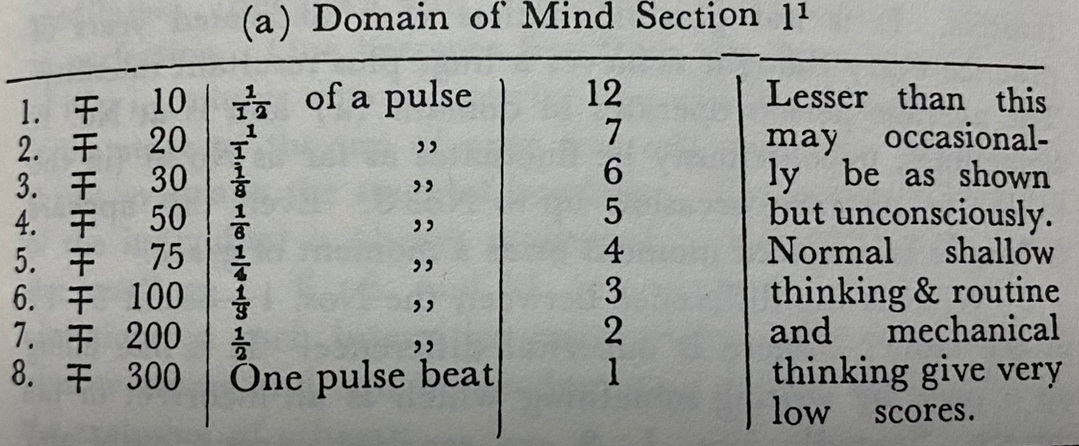
\includegraphics[width=0.9\linewidth,keepaspectratio]{images/zenyoga3}
	\end{center}
	
1st row, in 1 pulse, usually you get 12 thoughts, there you get 10 zenyoga points. If you get 1 thoughts per pulse (last row), then you get 300 points. 3SRB way is to reduce thoughts per pulse. Saving energy needed to decode those many thoughts.

\end{frame}

%%%%%%%%%%%%%%%%%%%%%%%%%%%%%%%%%%%%%%%%%%%%%%%%%%%%%%%%%%%%%%%%
\begin{frame}[fragile]\frametitle{Thoughts per Pulse}
	\begin{center}
	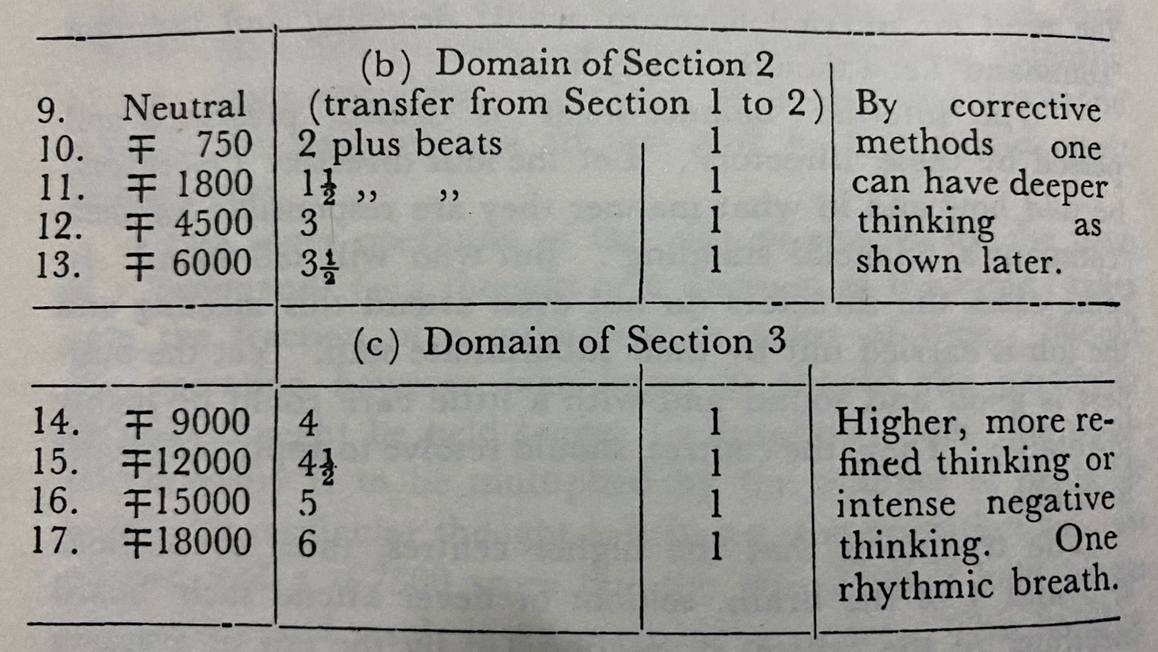
\includegraphics[width=0.9\linewidth,keepaspectratio]{images/zenyoga4}
	\end{center}
	
Reaching CSS you can hold 1 thought for 2-3-6 pulses.

\end{frame}

%%%%%%%%%%%%%%%%%%%%%%%%%%%%%%%%%%%%%%%%%%%%%%%%%%%%%%%%%%%%%%%%
\begin{frame}[fragile]\frametitle{Energy Drain and Thought Frequency}
    \begin{itemize}
        \item High thought-decoding rate exhausts mental and physical energy.
        \item An average person decodes approximately 51,000 thoughts per hour.
        \item Unconscious impulses from the five senses contribute to this high volume.
    \end{itemize}
\end{frame}

%%%%%%%%%%%%%%%%%%%%%%%%%%%%%%%%%%%%%%%%%%%%%%%%%%%%%%%%%%%%%%%%
\begin{frame}[fragile]\frametitle{Reducing Thought Frequency for Greater Intensity}
    \begin{itemize}
        \item Reducing thought frequency increases resultant intensity.
        \item Focus on breathing techniques, especially Three-Step Breathing, to slow down thought frequency.
        \item Slower frequency enhances mental clarity and reserves energy for higher purposes.
    \end{itemize}
\end{frame}

%%%%%%%%%%%%%%%%%%%%%%%%%%%%%%%%%%%%%%%%%%%%%%%%%%%%%%%%%%%%%%%%
\begin{frame}[fragile]\frametitle{Role of Heartbeat and Breathing in Thought Decoding}
    \begin{itemize}
        \item Thought decoding links to heartbeat and pulse frequency.
        \item Normal pulse rate allows decoding at a slower, more sustainable pace.
        \item Breathing practices help normalize pulse, stabilizing thought processes.
    \end{itemize}
\end{frame}

%%%%%%%%%%%%%%%%%%%%%%%%%%%%%%%%%%%%%%%%%%%%%%%%%%%%%%%%%%%%%%%%
\begin{frame}[fragile]\frametitle{Three-Step Breathing for Mental Calm}
    \begin{itemize}
        \item Three-Step Breathing helps in regulating the pulse to an ideal rate of 72 beats per minute.
        \item Reduces thought frequency, allowing energy conservation.
        \item Aids in gathering and storing Zen Yoga units effectively.
    \end{itemize}
\end{frame}

%%%%%%%%%%%%%%%%%%%%%%%%%%%%%%%%%%%%%%%%%%%%%%%%%%%%%%%%%%%%%%%%
\begin{frame}[fragile]\frametitle{Advanced Sections of the Mind}
    \begin{itemize}
        \item Sections 2, 3, and 4 of the mind require deeper thought regulation.
        \item Higher sections enable more intense thought folding per pulse.
        \item Advanced levels are only accessible with critical mastery of thought and pulse control.
    \end{itemize}
\end{frame}

%%%%%%%%%%%%%%%%%%%%%%%%%%%%%%%%%%%%%%%%%%%%%%%%%%%%%%%%%%%%%%%%
\begin{frame}[fragile]\frametitle{Section 2 Thought Decoding}
    \begin{itemize}
        \item As frequency reduces, thoughts fold into fewer pulses.
        \item Section 2 enables gathering up to 750 units of resultant intensity.
        \item Progressing beyond Section 1 requires substantial reduction in thought frequency.
    \end{itemize}
\end{frame}

%%%%%%%%%%%%%%%%%%%%%%%%%%%%%%%%%%%%%%%%%%%%%%%%%%%%%%%%%%%%%%%%
\begin{frame}[fragile]\frametitle{Zen Yoga Unit Collection in Higher Mind Sections}
    \begin{itemize}
        \item Mind sections gather specific intensities based on decoding frequency.
        \item Higher sections (3 and 4) allow folding of thoughts over multiple pulses, enhancing intensity.
        \item Advanced breathing and pulse control lead to refined positive or negative unit collection.
    \end{itemize}
\end{frame}

%%%%%%%%%%%%%%%%%%%%%%%%%%%%%%%%%%%%%%%%%%%%%%%%%%%%%%%%%%%%%%%%
\begin{frame}[fragile]\frametitle{Practical Application of Three-Step Breathing}
    \begin{itemize}
        \item Dedicate 10-15 minutes daily to Three-Step Breathing.
        \item Practice reduces unnecessary thoughts and energy drain.
        \item Regular practice aligns pulse and thought rates, conserving mental and physical energy.
    \end{itemize}
\end{frame}

%%%%%%%%%%%%%%%%%%%%%%%%%%%%%%%%%%%%%%%%%%%%%%%%%%%%%%%%%%%%%%%%
\begin{frame}[fragile]\frametitle{Conclusion: Evolving Through Zen Yoga}
    \begin{itemize}
        \item Zen Yoga emphasizes reducing thought frequency to achieve deeper mental states.
        \item Regulated pulse and breathing stabilize mental processes, making higher mind sections accessible.
        \item Mastery in thought control allows for Zen Yoga units to transform into positive, enduring energy.
    \end{itemize}
\end{frame}

%%%%%%%%%%%%%%%%%%%%%%%%%%%%%%%%%%%%%%%%%%%%%%%%%%%%%%%%%%%%%%%%
\begin{frame}[fragile]\frametitle{}
\begin{center}
{\Large Chapter 11: Use of Free Will in Trifles }
\end{center}
\end{frame}

%%%%%%%%%%%%%%%%%%%%%%%%%%%%%%%%%%%%%%%%%%%%%%%%%%%%%%%%%%%%%%%%
\begin{frame}[fragile]\frametitle{Use of Free Will and False Choices}
    \begin{itemize}
        \item Discussion on free will and how humans exercise it.
        \item Zenyoga emphasizes utilizing free will for spiritual growth.
        \item Importance of making conscious choices that align with life's purpose.
    \end{itemize}
\end{frame}

%%%%%%%%%%%%%%%%%%%%%%%%%%%%%%%%%%%%%%%%%%%%%%%%%%%%%%%%%%%%%%%%
\begin{frame}[fragile]\frametitle{Yoga's Eight Limbs}
    \begin{itemize}
        \item Zenyoga introduces the eight limbs of Yoga as steps toward enlightenment.
        \item Key stages: Yama, Niyama, Asana, Pranayama, Pratyahara, Dharana, Dhyana, Samadhi. यम नियम आसन प्राणायाम प्रत्याहार धारणा ध्यान समाधी 
        \item Final three stages focus on concentration, meditation, and transcendent union.
    \end{itemize}
\end{frame}

%%%%%%%%%%%%%%%%%%%%%%%%%%%%%%%%%%%%%%%%%%%%%%%%%%%%%%%%%%%%%%%%
\begin{frame}[fragile]\frametitle{Self-Discipline and Habit Formation}
    \begin{itemize}
        \item Yama, Niyama, Asana, and Pranayama यम नियम आसन प्राणायाम promote self-discipline in daily habits.
        \item Moderation in all activities, including eating and sleeping, is essential.
        \item Overindulgence affects physical and spiritual growth, slowing progress.
    \end{itemize}
\end{frame}

%%%%%%%%%%%%%%%%%%%%%%%%%%%%%%%%%%%%%%%%%%%%%%%%%%%%%%%%%%%%%%%%
\begin{frame}[fragile]\frametitle{Pratyahara – Withdrawal of Senses}
    \begin{itemize}
        \item Pratyahara प्रत्याहार is the stage of withdrawing from sensory distractions.
        \item Achieving this step fosters self-awareness beyond the physical body.
        \item It prepares the mind for deeper states of meditation.
    \end{itemize}
\end{frame}

%%%%%%%%%%%%%%%%%%%%%%%%%%%%%%%%%%%%%%%%%%%%%%%%%%%%%%%%%%%%%%%%
\begin{frame}[fragile]\frametitle{Role of Moderation in Daily Activities}
    \begin{itemize}
        \item Zenyoga emphasizes moderation in food, sleep, and all daily activities.
        \item Excess in any aspect leads to negative effects on body and mind.
        \item "Disinfection Chamber" approach: a disciplined boundary for actions.
    \end{itemize}
\end{frame}

%%%%%%%%%%%%%%%%%%%%%%%%%%%%%%%%%%%%%%%%%%%%%%%%%%%%%%%%%%%%%%%%
\begin{frame}[fragile]\frametitle{Understanding True Free Will}
    \begin{itemize}
        \item Misinterpretation of free will often leads to impulsive actions.
        \item Zenyoga teaches discerning right actions that contribute to spiritual growth.
        \item Avoid actions solely for temporary pleasures that detract from growth.
    \end{itemize}
\end{frame}

%%%%%%%%%%%%%%%%%%%%%%%%%%%%%%%%%%%%%%%%%%%%%%%%%%%%%%%%%%%%%%%%
\begin{frame}[fragile]\frametitle{Addictions and Misuse of Free Will}
    \begin{itemize}
        \item Addictions hinder spiritual and personal growth.
        \item Zenyoga addresses overcoming habits like overeating, substance use, and excessive sleep.
        \item Self-awareness and mindful action are essential to overcoming these patterns.
    \end{itemize}
\end{frame}

%%%%%%%%%%%%%%%%%%%%%%%%%%%%%%%%%%%%%%%%%%%%%%%%%%%%%%%%%%%%%%%%
\begin{frame}[fragile]\frametitle{Mind and Breath Control}
    \begin{itemize}
        \item Breath awareness is crucial for mental clarity and spiritual well-being.
        \item Optimal breathing frequency affects mental stability and thought quality.
        \item Nose breathing is recommended over mouth breathing for health and mental focus.
    \end{itemize}
\end{frame}

%%%%%%%%%%%%%%%%%%%%%%%%%%%%%%%%%%%%%%%%%%%%%%%%%%%%%%%%%%%%%%%%
\begin{frame}[fragile]\frametitle{Quality of Thoughts and Diet}
    \begin{itemize}
        \item Zenyoga highlights the connection between diet and quality of thoughts.
        \item Consumption of natural, balanced foods promotes positive, clear thoughts.
        \item Tamasik (heavy) foods tend to generate lethargic, negative thoughts.
    \end{itemize}
\end{frame}

%%%%%%%%%%%%%%%%%%%%%%%%%%%%%%%%%%%%%%%%%%%%%%%%%%%%%%%%%%%%%%%%
\begin{frame}[fragile]\frametitle{Life and Spiritual Journey Alignment}
    \begin{itemize}
        \item Zenyoga aims to harmonize physical habits with spiritual goals.
        \item Thoughtful habits and balanced choices lead to sustained growth.
        \item Recognizing the impact of actions today on future well-being.
    \end{itemize}
\end{frame}


%%%%%%%%%%%%%%%%%%%%%%%%%%%%%%%%%%%%%%%%%%%%%%%%%%%%%%%%%%%%%%%%
\begin{frame}[fragile]\frametitle{}
\begin{center}
{\Large Chapter 12: Corrective Methods In Daily Living }
\end{center}
\end{frame}

%%%%%%%%%%%%%%%%%%%%%%%%%%%%%%%%%%%%%%%%%%%%%%%%%%%%%%%%%%%%%%%%
\begin{frame}[fragile]\frametitle{Corrective Methods in Daily Living}
    \begin{itemize}
        \item The chapter discusses corrective methods in daily activities essential for survival.
        \item Focus on understanding common errors in daily actions and the correct approaches.
        \item Main topics include:
        \begin{itemize}
            \item Food and Drink
            \item Breath (Prana)
            \item Sensory Inputs and Thought Generation
        \end{itemize}
    \end{itemize}
\end{frame}

%%%%%%%%%%%%%%%%%%%%%%%%%%%%%%%%%%%%%%%%%%%%%%%%%%%%%%%%%%%%%%%%
\begin{frame}[fragile]\frametitle{Food and Drink: Mindful Consumption}
    \begin{itemize}
        \item Avoid preconceptions about vegetarian vs. non-vegetarian food.
        \item Choose foods that are easy for the body to digest.
        \item Maintain a calm mind while eating; express gratitude for the sustenance.
        \item Young individuals (below 21 years) may consume freely due to growth needs.
        \item For adults, focus on maintenance, replacing old cells, and restoring energy levels.
    \end{itemize}
\end{frame}

%%%%%%%%%%%%%%%%%%%%%%%%%%%%%%%%%%%%%%%%%%%%%%%%%%%%%%%%%%%%%%%%
\begin{frame}[fragile]\frametitle{Eating Habits for Health}
    \begin{itemize}
        \item Gradually reduce food quantity if eating multiple times a day.
        \item Avoid eating before 10:00 AM; limit eating times between 10:00 AM and 4:00 PM.
        \item Reducing food quantity can lead to increased energy and lighter body sensations.
        \item Reduce food intake mindfully over time for sustainable change.
    \end{itemize}
\end{frame}

%%%%%%%%%%%%%%%%%%%%%%%%%%%%%%%%%%%%%%%%%%%%%%%%%%%%%%%%%%%%%%%%
\begin{frame}[fragile]\frametitle{Managing Energy and Reducing Food Needs}
    \begin{itemize}
        \item Energy drains from mental, sensory, and physical activities increase food and sleep needs.
        \item Conserving energy can lead to reduced food and sleep requirements.
        \item With reduced energy drain, fewer meals and less sleep can still maintain high energy.
    \end{itemize}
\end{frame}

%%%%%%%%%%%%%%%%%%%%%%%%%%%%%%%%%%%%%%%%%%%%%%%%%%%%%%%%%%%%%%%%
\begin{frame}[fragile]\frametitle{Personal Experimentation with Food Quantity}
    \begin{itemize}
        \item Gradually reduced meal size from five rotis to two or three without health effects.
        \item Evening meals are taken early to reduce body load, improving energy levels and reducing sleep needs.
        \item Experimenting over several years has shown no decline in health with reduced quantity.
    \end{itemize}
\end{frame}

%%%%%%%%%%%%%%%%%%%%%%%%%%%%%%%%%%%%%%%%%%%%%%%%%%%%%%%%%%%%%%%%
\begin{frame}[fragile]\frametitle{Drinking: The Ideal Choice}
    \begin{itemize}
        \item Water is the best drink for hydration.
        \item Avoid alcohol due to its harmful effects on body cells and organs.
        \item Keep the body energized with simple, easily digestible food and clean water.
    \end{itemize}
\end{frame}

%%%%%%%%%%%%%%%%%%%%%%%%%%%%%%%%%%%%%%%%%%%%%%%%%%%%%%%%%%%%%%%%
\begin{frame}[fragile]\frametitle{Introduction to Rhythmic Breathing}
    \begin{itemize}
        \item Importance of breathing rhythm for overall well-being.
        \item Rhythmic breathing method introduced to correct disrupted breathing.
        \item Inspired by natural breathing patterns observed in infants.
    \end{itemize}
\end{frame}

%%%%%%%%%%%%%%%%%%%%%%%%%%%%%%%%%%%%%%%%%%%%%%%%%%%%%%%%%%%%%%%%
\begin{frame}[fragile]\frametitle{Step 1: Focus on Technique}
    \begin{itemize}
        \item Emphasize natural breathing rhythm.
        \item Use a heavy book on the abdomen to monitor abdominal movement.
        \item Breathe through the nose to direct air into the lungs.
        \item Minimize chest movement to encourage deep lung expansion.
    \end{itemize}
\end{frame}

%%%%%%%%%%%%%%%%%%%%%%%%%%%%%%%%%%%%%%%%%%%%%%%%%%%%%%%%%%%%%%%%
\begin{frame}[fragile]\frametitle{Step 2: Focus on Volume}
    \begin{itemize}
        \item Concentrate on filling the lungs completely.
        \item Practice against a wall with hands placed upwards to open the chest.
        \item Learn to increase air volume in each breath cycle.
        \item Maintain focus on proper lung expansion.
    \end{itemize}
\end{frame}

%%%%%%%%%%%%%%%%%%%%%%%%%%%%%%%%%%%%%%%%%%%%%%%%%%%%%%%%%%%%%%%%
\begin{frame}[fragile]\frametitle{Step 3: Natural Rhythm}
    \begin{itemize}
        \item Combine techniques from Steps 1 and 2.
        \item Breathing aligns with natural, relaxed rhythm.
        \item Practicing for 6+ months leads to unconscious mastery.
        \item Achieve lower heart and breath rates, indicating improved calmness.
    \end{itemize}
\end{frame}

%%%%%%%%%%%%%%%%%%%%%%%%%%%%%%%%%%%%%%%%%%%%%%%%%%%%%%%%%%%%%%%%
\begin{frame}[fragile]\frametitle{Benefits of Rhythmic Breathing Practice}
    \begin{itemize}
        \item Reduced irritability and stress response.
        \item Enhanced mental clarity and focus.
        \item Greater control over emotional responses.
        \item Improved physical and mental resilience in daily life.
    \end{itemize}
\end{frame}

%%%%%%%%%%%%%%%%%%%%%%%%%%%%%%%%%%%%%%%%%%%%%%%%%%%%%%%%%%%%%%%%
\begin{frame}[fragile]\frametitle{Not Pranayama, but a Pre-Practice}
    \begin{itemize}
        \item Rhythmic breathing is not Pranayama.
        \item Suitable for those at preliminary stages of breathing practice.
        \item Focuses on rhythm and volume before advancing to Pranayama.
    \end{itemize}
\end{frame}
